\section{Overview}
\label{sec: overview}%
In this section, a general description of the architecture of the \verb|eMALL| system is provided.
The main aspects of the design are:
\begin{itemize}
    \item \textbf{Client-Server architecture. } It consists of a presentation tier, an application and a data tier.
    The firsts one allow the user to communicate with the server and shows him through the UI the answers it receives back from the application tier.
    The second one receives requests from users, elaborates answers, changes the status communicating with the data tier and sends back the needed information to users.
    Finally, the data tier stores, updates, and handles the information.
    \item \textbf{Microservices. } Functionalities of the system are divided into several services in order to reduce dependencies between
    modules and to increase scalability, availability and maintainability of the system.
\end{itemize}
Detailed description of the features of the architecture will be provided in the next sections.

\newpage


\section{Component View}
\label{sec: component_view}%
The component diagram shows all the identified components.
It also describes the relations between the modules, representing the verse of the communication flow and the actors of it.
Before showing the diagram, there must be clarifications about it:
\begin{itemize}
    \item Two client applications are represented, one for both EVD and CPO. They are the same client application.
    We preferred to double the module in the diagram to facilitate comprehension of how users communicate with the system.
    \item For the same reasons, there are duplicated interfaces offered by components.
    \item The diagram shows a macro component called \verb|eMALL| that represents the whole system.
    Outside the system, they are shown the external services, the DBMSs, and the client application.
    Communication between modules and \verb|eMALL| happens thanks to interfaces that the system offers or exploits, depending on the component.
\end{itemize}
After the diagram, it will follow a brief description of each identified component.

\subsection{Component diagram}
\label{subsec:component_diagram}%
\begin{figure} [H]
    \begin{center}
        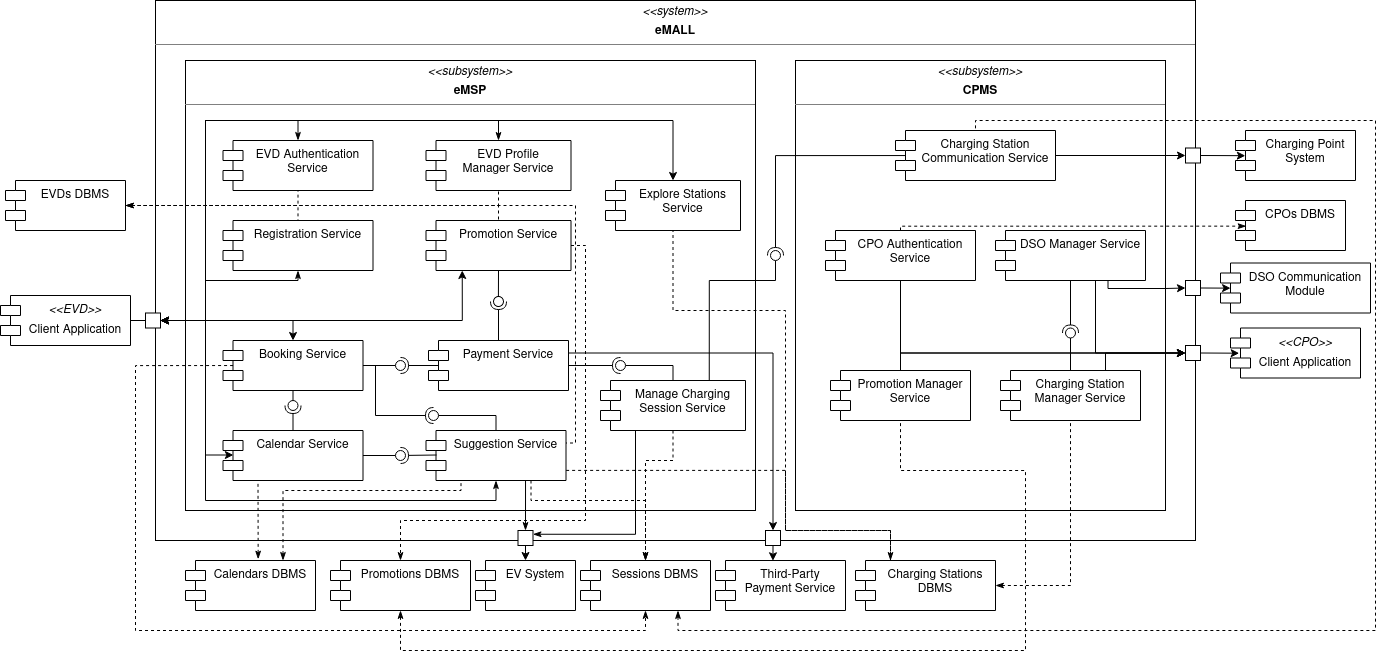
\includegraphics[width=1\linewidth]{ComponentDiagram/component_diagram}
        \caption{Component diagram of the eMALL system.}
        \label{fig: cd}
    \end{center}
\end{figure}

\subsection{Components description}
\label{subsec:components_description}%
The components are:
\begin{itemize}
    \item \textbf{Client Application.} \verb|Client| \verb|Application| represent the client system used to connect and to communicate
    with \verb|eMALL|.
    \item \textbf{Registration Service.} \verb|Registration| \verb|Service| handles the process of the creation
    of a new account requested by a new EVD user.
    It communicates with \verb|EVDs| \verb|DBMS| to save the information about the new created account.
    \item \textbf{EVD Authentication Service.} \verb|EVD| \verb|Authentication| \verb|Service| handles the login process requested by an EVD\@.
    To do that, it communicates with \verb|EVDs| \verb|DBMS| to validate the inserted credentials.
    \item \textbf{EVD Profile Manager Service.} \verb|EVD| \verb|Profile| \verb|Manager| \verb|Service| offers the possibility to query
    the \verb|EVDs| \verb|DBMS| in order to get requested information.
    In general, it is the service offered to the user to get or update information of the profile.
    So, he communicates with \verb|EVDs| \verb|DBMS|.
    \item \textbf{Explore Stations Service.} \verb|Explore| \verb|Stations| \verb|Service| is the service used by the EVDs to navigate
    into the map of charging station that can be found around user's position.
    To do that, he needs stations position, so it communicates with \verb|Charging| \verb|Stations| \verb|DBMS|.
    Furthermore, it communicates also with the external service \verb|Navigator| \verb|System|, used to elaborate positions
    and to show them into the map.
    \item \textbf{Booking Service.} \verb|Booking| \verb|Service| is the module used to handle booking requests.
    It communicates with \verb|Sessions| \verb|DBMS| to save the information about bookings and with \verb|Calendar| \verb|Service|
    to start the process of insertion of a new activity into EVD's calendar representing the booked reservation.
    \item \textbf{Manage Charging Session Service.} \verb|Manage| \verb|Charging| \verb|Session| \verb|Service| handles the charging session process.
    It allows the EVDs to start and interrupt the session and to pay for the service the user enjoyed.
    Furthermore, it sends to the EVDs notifications about ongoing session status.
    The module communicates with \verb|Charging| \verb|Station| \verb|Communication| \verb|Service| to delegate the communication with the charging point
    where the EVD wants to charge the EV\@.
    As said before, the service offers the EVD the interface to make the payment of the session, so it communicates with
    \verb|Payment Service|.
    After the payment, the module saves the receipt of the session communicating the \verb|Sessions| \verb|DBMS| module.
    \item \textbf{Promotion Service.} \verb|Promotion| \verb|Service| offers the EVDs the possibility to activate special promotions
    activated by CPOs.
    To get the list of active promotions, it communicates with \verb|Promotions| \verb|DBMS|.
    The module communicates also with \verb|EVD| \verb|Profile| \verb|Manager| \verb|Service| to delegate the save of the activation of a special offer into
    the \verb|EVDs DBMS|.
    \item \textbf{Calendar Service.} \verb|Calendar| \verb|Service| is module that manages EVDs calendar.
    It offers the possibility to visualize the calendar, saved events and their details.
    It also offers the functionality of activity insertion.
    To save all this information, the module communicates with \verb|Calendars| \verb|DBMS|.
    After a new activity is inserted, \verb|Calendar| \verb|Service| activates the process offered by \verb|Suggestion| \verb|Service|
    in order to create suggestion about when and where the EVD should charge the EV\@.
    \item \textbf{Suggestion Service.} \verb|Suggestion| \verb|Service| communicates with different modules to create suggestions.
    It communicates with:
    \begin{itemize}
        \item \verb|EVDs| \verb|DBMS| to get user's EV specifications.
        \item \verb|Calendar| \verb|DBMS| to get EVD's schedule to know precedent events that could affect the research.
        \item \verb|EV| \verb|System| to get current EV status.
        \item \verb|Charging| \verb|Stations| \verb|DBMS| to get positions of the memorized charging stations.
        \item \verb|Navigation| \verb|System| to calculate the path between the positions defined in the schedule of the EVD,
        and to identify which charging stations can be suggested to the user.
        \item \verb|Sessions| \verb|DBMS| to get schedules of the charging point, getting in this way their available timeframes,
        and to see if there are other bookings done by the EVD\@.
        \item \verb|Booking| \verb|Service| to start the booking process after the EVD confirms the received suggestion.
    \end{itemize}
    \item \textbf{Payment Service.} \verb|Payment| \verb|Service| offers the possibility to pay for a service the EVD enjoyed.
    It communicates with \verb|EVD| \verb|Profile| \verb|Manager| \verb|Service| to get EVD's payment methods.
    Once it has the needed information, it communicates with \verb|Third-Party| \verb|Payment| \verb|Service| to make the payment.
    \item \textbf{CPO Authentication Service.} \verb|CPO| \verb|Authentication| \verb|Service| handles the login process requested by a CPO\@.
    To do that, it communicates with \verb|CPOs| \verb|DBMS| to validate the inserted credentials.
    \item \textbf{CPO Profile Manager Service.} \verb|CPO| \verb|Profile| \verb|Manager| \verb|Service| offers the possibility to query
    the \verb|CPOs| \verb|DBMS| in order to get requested information.
    In general, it is the service offered to the user to get or update information of the profile.
    So, he communicates with \verb|CPOs| \verb|DBMS|.
    \item \textbf{Charging Station Manager Service.} \verb|Charging| \verb|Station| \verb|Manager| \verb|Service| is the service offered to CPOs
    to manage their charging stations and their charging points.
    One of the functionalities is to plan a maintenance session for a charging station.
    To do that, the module communicates with the \verb|Charging| \verb|Station| \verb|Communication| \verb|Service| module.
    Finally, it communicates with \verb|Charging| \verb|Stations| \verb|DBMS| to store the information.
    \item \textbf{Charging Station Communication Service.} \verb|Charging| \verb|Station| \verb|Communication| \verb|Service| is the module
    that communicates with charging points.
    Messages are exchanged when an EVD starts or ends the charging session or when the CPO plans a maintenance session.
    \item \textbf{Promotion Manager Service.} \verb|Promotion| \verb|Manager| \verb|Service| is used by CPOs to manage their promotions.
    The module communicates with \verb|Promotions| \verb|DBMS| to save or update promotions information.
    \item \textbf{DSO Manager Service.} \verb|DSO| \verb|Manager| \verb|Service| is the module aimed for the communication with DSOs.
    To do that, it exchanges messages with the external service \verb|DSO| \verb|Communication| \verb|Module|.
    When a CPO decides to change its electricity provider, the module delegates \verb|CPO| \verb|Profile| \verb|Manager| \verb|Service| to
    save the information into the \verb|CPOs| \verb|DBMS|.
    \item \textbf{EVDs DBMS.} \verb|EVDs| \verb|DBMS| is the system used to save all the information about EVDs, such as
    credentials, EVs, active promotions.
    \item \textbf{Calendars DBMS.} \verb|Calendars| \verb|DBMS| is the system used to save all the information about activities
    inserted by EVDs and to save location and hour of a booked charging session.
    In this way, it is easily obtainable by the EVD\@.
    \item \textbf{Sessions DBMS.} \verb|Sessions| \verb|DBMS| is the system used to save information about bookings
    specifying data that would be useless for the EVD\@.
    It is also used to save the receipts of the charging sessions done by the EVDs.
    \item \textbf{CPOs DBMS.} \verb|CPOs| \verb|DBMS| is the system used to save all the information about CPOs, such as credentials,
    company information.
    \item \textbf{Charging Stations DBMS.} \verb|Charging| \verb|Stations| \verb|DBMS| is the system used to save the information about
    charging stations and charging points.
    \item \textbf{Promotions DBMS.} \verb|Promotions| \verb|DBMS| is the system used to save information about promotions
    that have been activated by the CPOs.
    \item \textbf{EV System.} \verb|EV| \verb|system| is an external service that gives the system the possibility to retrieve
    information about EVDs EV\@.
    \item \textbf{Navigator System.} \verb|Navigator| \verb|System| is an external service that gives the system the possibility
    to work on positions and elaborate paths between locations.
    \item \textbf{Third-Party Payment Service.} \verb|Third-Party| \verb|Payment| \verb|Service| is an external service used to
    make payments communicating with banks or payment sites.
    \item \textbf{Charging Point System.} \verb|Charging| \verb|Point| \verb|System| is an external service that represent the software
    running on charging points.
    It is used in the CPOs interactions to manage their charging points.
    \item \textbf{DSO Communication Module.} \verb|DSO| \verb|Communication| \verb|Module| is an external service that gives the system
    to communicate with the DSOs in order to get their prices and to enable electricity providing.
\end{itemize}

\newpage


\section{Deployment View}
\label{sec: deployment_view}%
The following deployment diagram shows how all the components are distributed into different nodes,
highlighting how they communicate with each other. \\
The next paragraphs will go into details about the reasons behind the design choices. \\
The deployment diagram is:
\begin{figure} [H]
    \begin{center}
        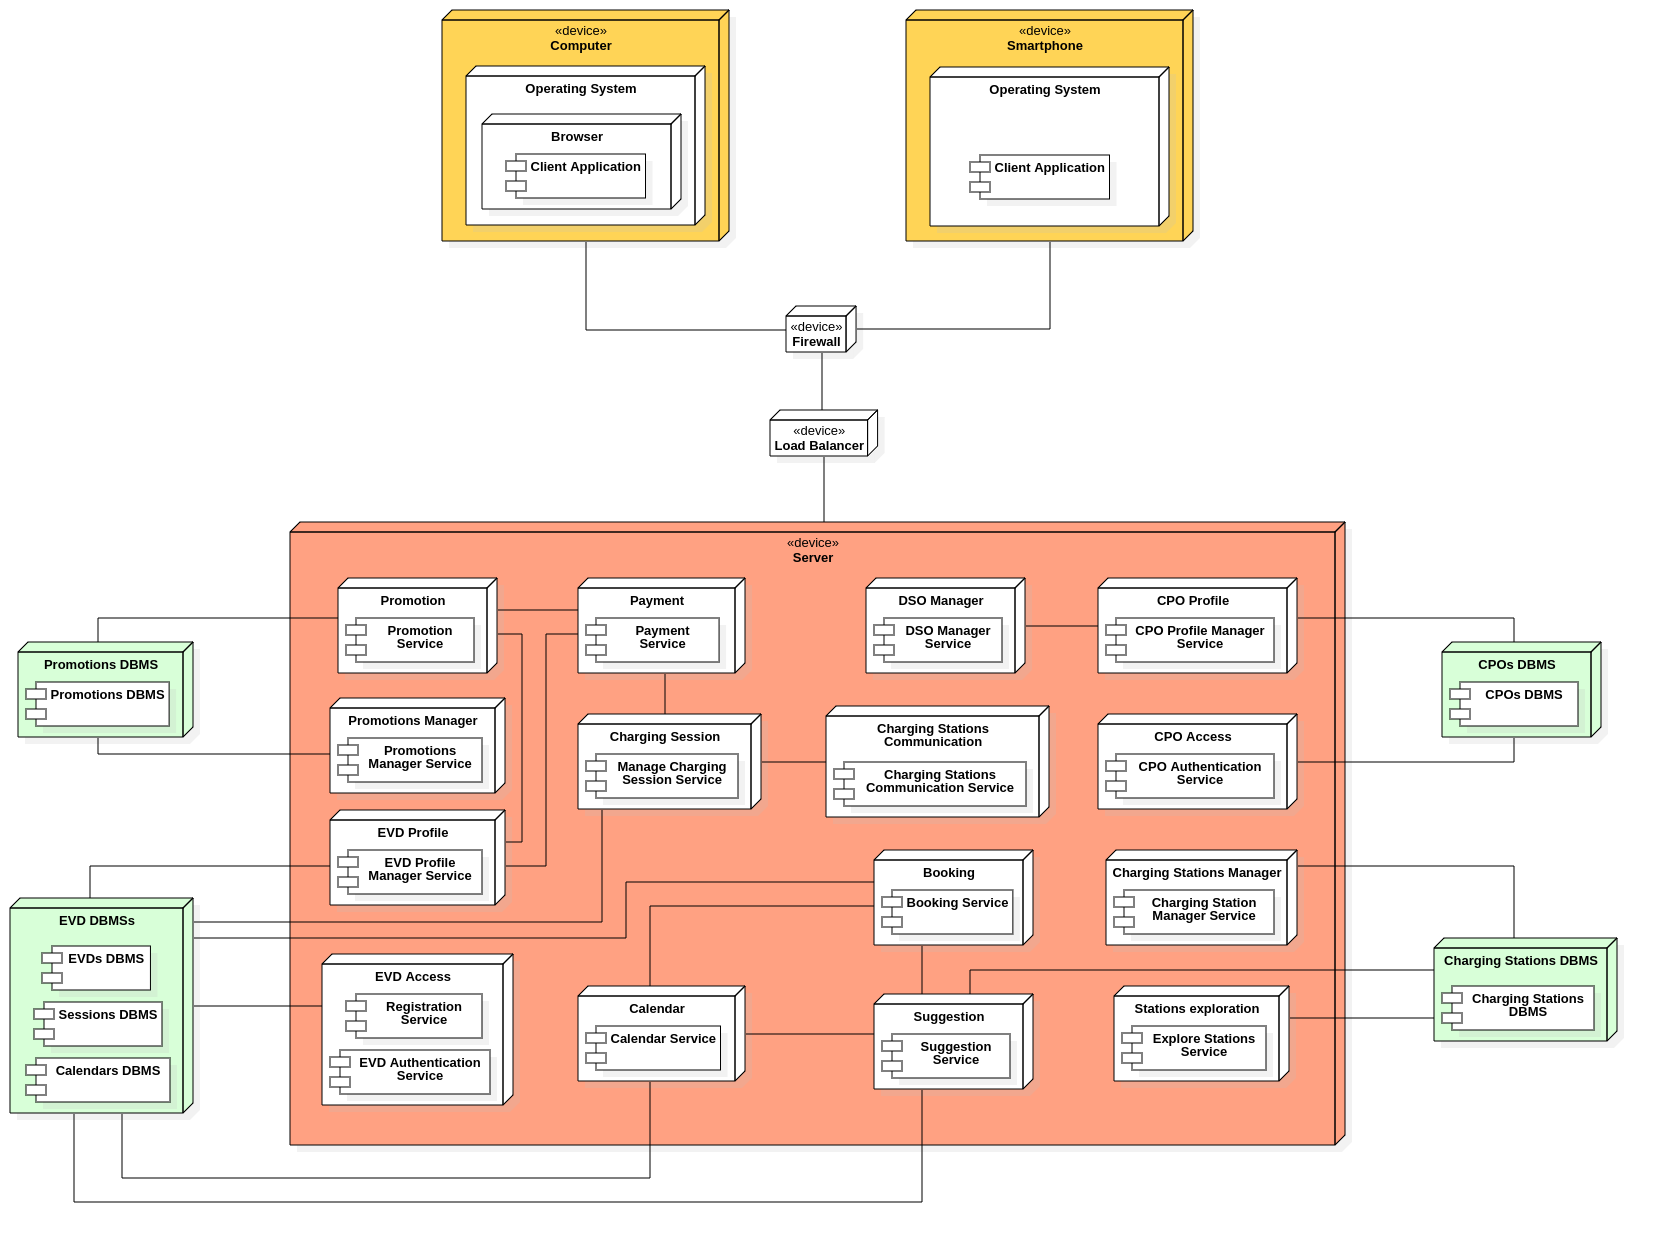
\includegraphics[width=1\linewidth]{DeploymentDiagram/deployment_diagram}
        \caption{Deployment diagram of the eMALL system.}
        \label{fig: depl_diagram}
    \end{center}
\end{figure}

\subsection{Connection to the server}
\label{subsec:connection_to_the_server}%
EVDs and CPOs can access the eMALL system from both PC and smartphones.
In the first case, it is necessary to use a browser to load the system's web page.
In the second case, the client will use the application after downloading it from the smartphone's store (Android or iOS).
When requests are sent to the server, first they pass into the firewall, so to avoid eventual cyberattacks on the system,
then they pass into the load balancer, so to optimize resource usage,
improve performance, and increase the availability of several services.
Requests are now ready to be handled by the eMALL services. \\
It follows the corresponding part from the deployment diagram:
\begin{figure} [H]
    \begin{center}
        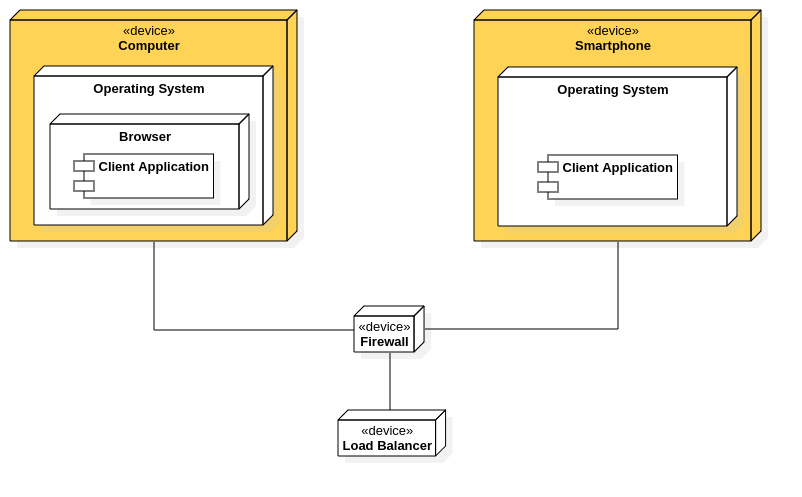
\includegraphics[width=0.7\linewidth]{DeploymentDiagram/connection}
        \caption{Connection to the server diagram.}
        \label{fig: connection}
    \end{center}
\end{figure}

\subsection{Promotions}
\label{subsec:promotions}%
Promotion DBMS is one of the four identified DBMS nodes.
The choice of dividing it from other DBMSs relies on the will to better scale the system.
In this way, it is easier to guarantee the availability of other services that don't work with promotions,
and maintenance sessions are facilitated too.
It has not been grouped with other DBMSs into the same node because Promotions DBMS is also used by CPOs,
so the system needs to guarantee a high level of scalability to assure business functionalities to the companies. \\
It follows the corresponding part from the deployment diagram:
\begin{figure} [H]
    \begin{center}
        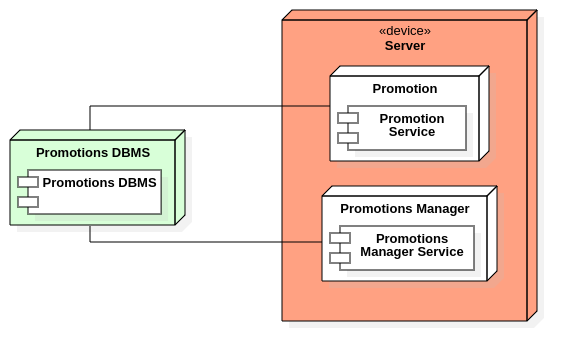
\includegraphics[width=0.6\linewidth]{DeploymentDiagram/promotion}
        \caption{Promotions managing diagram.}
        \label{fig: promotion}
    \end{center}
\end{figure}

\subsection{EVD interactions}
\label{subsec:evd_interactions}%
This section shows how the system communicates with \verb|EVDs DBMS|\@.
We choose to group \verb|EVDs DBMS|, \verb|Sessions DBMS|, and \verb|Calendars DBMS| into the same node because
they all receive requests from the services only in case of interactions with EVDs.
Considering that they don't introduce strict time response requirements,
it was not necessary to insert new physical nodes for the managing of the DBMSs. \\
It follows the corresponding part from the deployment diagram:
\begin{figure} [H]
    \begin{center}
        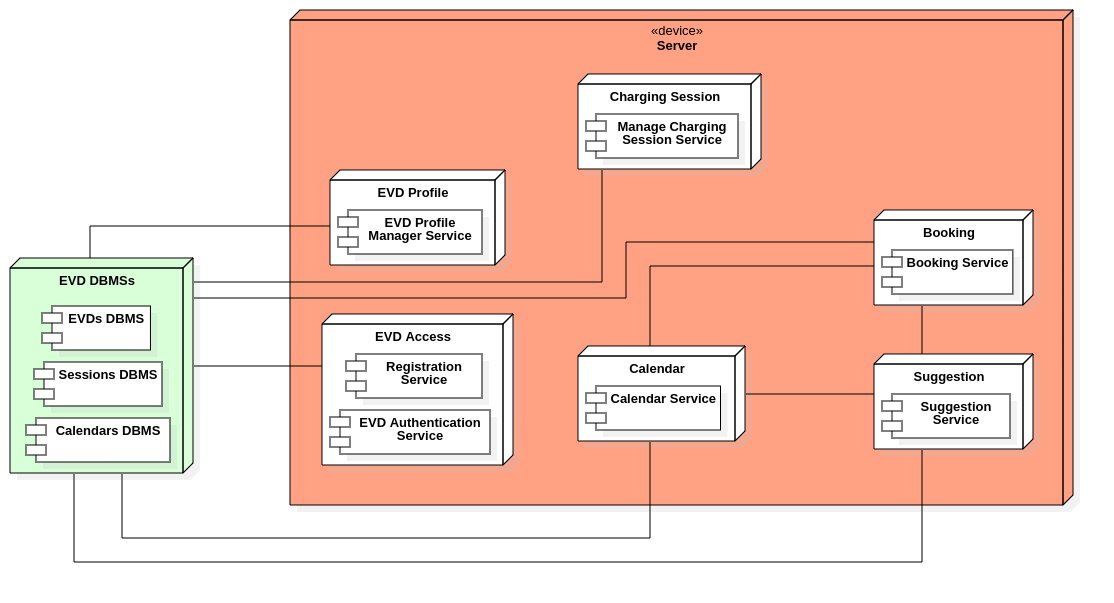
\includegraphics[width=\linewidth]{DeploymentDiagram/EVD_interactions}
        \caption{EVD interactions diagram.}
        \label{fig: evd_interactions}
    \end{center}
\end{figure}

\subsection{CPOs DBMS}
\label{subsec:cpo_dbms}%
The components that communicate with the CPOs DBMS are the Authentication Service and the CPO Profile Manager Service.
When another service needs to get or to update information about a CPO, the request is handled by the CPO Profile node.
The DBMS is used by CPOs, so it is deployed in a single node to better scale the system,
and to guarantee business functionalities to the companies. \\
It follows the corresponding part from the deployment diagram:
\begin{figure} [H]
    \begin{center}
        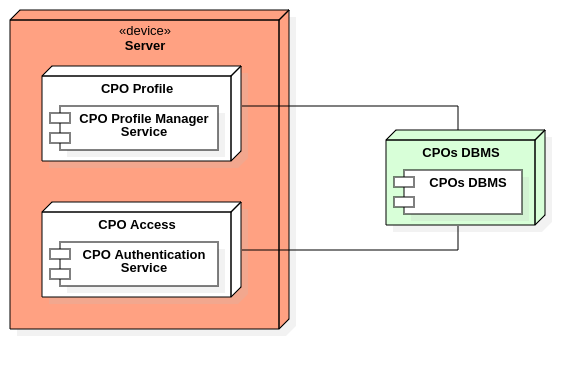
\includegraphics[width=0.6\linewidth]{DeploymentDiagram/CPO_DBMS}
        \caption{CPOs DBMS managing diagram.}
        \label{fig: cpo_dbms}
    \end{center}
\end{figure}

\subsection{Charging stations communication}
\label{subsec:charging_stations_communication}%
Suggestion and Stations exploration nodes read from the DBMS
to get the position of the stations that will be elaborated or shown to the user.
Charging Station Manager Service can also write or update the instances of the DBMS\@.
The DBMS is used by CPOs, so it is deployed in a single node to better scale the system,
and to guarantee business functionalities to the companies. \\
It follows the corresponding part from the deployment diagram:
\begin{figure} [H]
    \begin{center}
        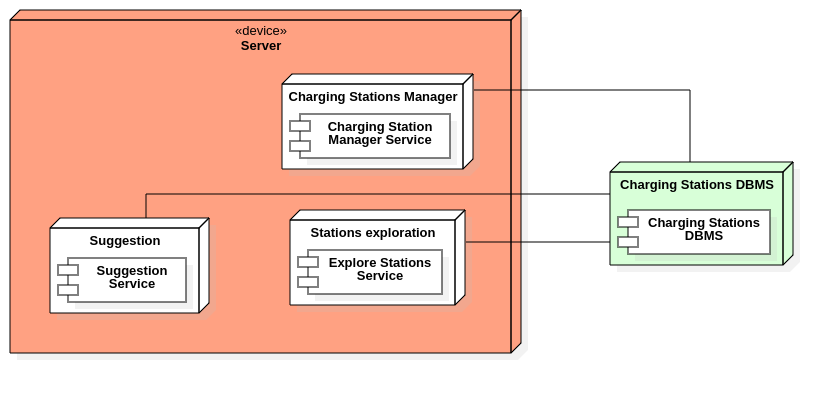
\includegraphics[width=0.85\linewidth]{DeploymentDiagram/charging_stations_communication}
        \caption{Charging stations communication diagram.}
        \label{fig: charing_stations_dbms}
    \end{center}
\end{figure}

\subsection{Services}
\label{subsec:services}%
The section shows all the identified nodes in which services run. \\
Decisions have been made giving particular attention to the concepts of loose coupling and high cohesion.
As explained in Sam Newman's \textit{Building Microservices}, they are defined as follows:
\begin{itemize}
    \item \textbf{Loose coupling.} \textit{When services are loosely coupled, a change to one service should not require a change to another.
    The whole point of a microservice is being able to make a change to one service and deploy it,
        without needing to change any other part of the system.}
    \item \textbf{High Cohesion.} \textit{We want related behavior to sit together, and unrelated behavior to sit elsewhere.
    Making changes in lots of different places is slower, and deploying lots of services at once is risky, both of which we want to avoid.}
\end{itemize}
The following image wants also to highlight the relations between different services, which are direct consequences of the
communication interfaces previously shown in the component diagram.
\begin{figure} [H]
    \begin{center}
        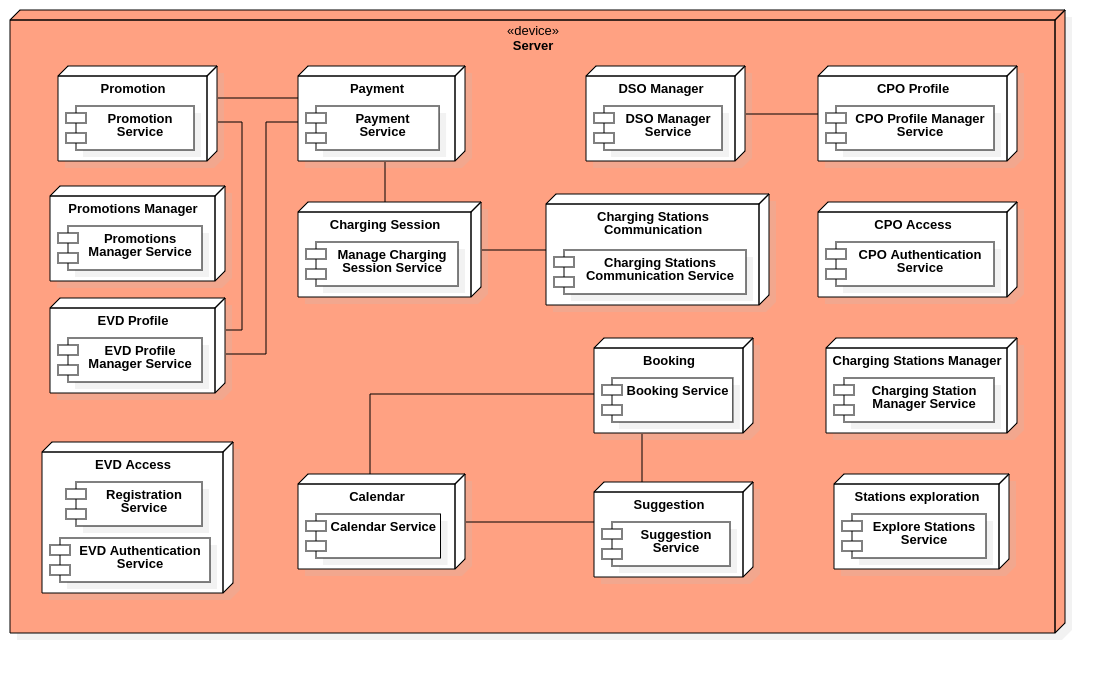
\includegraphics[width=\linewidth]{DeploymentDiagram/server}
        \caption{Server services diagram.}
        \label{fig: services}
    \end{center}
\end{figure}

\newpage


\section{Runtime View}
\label{sec:runtime_view}%
Here we present the dynamic of our system through sequence diagrams.
We have found the components that communicate with each other to form our system, so now we explain their behaviors.

First, we will present eMALL actions from the point of view of the EVD user, i.e., logging in, booking a charge, managing his profile, etc.
Then, we will present eMALL actions from the point of view of the CPO user, actions that are much more business functionality.
In this section, we hadn't presented all the RASD document use cases because we have decided to focus on the critical part of the system functionalities.

\paragraph{Registered EVD Logs In}
When the EVD - \verb|Client Application| - wants to log in to eMALL, he calls the ``\verb|logIn|'' function from the \verb|EVD| \verb|Authentication| \verb|Service| component.
That component requests the client to display the login form by running the ``\verb|displayLogInForm|'' function, and then it waits for the email and password from the \verb|Client| \verb|Application|.

When the EVD sends this information, the Authentication Service asks the \verb|EVDs| \verb|DBMS| to validate it.
Finished processing the login, the last component returns an ACK message to the \verb|EVD| \verb|Authentication| \verb|Service|, which sends a confirmation or an error to the client.
\begin{figure}[H]
    \begin{center}
        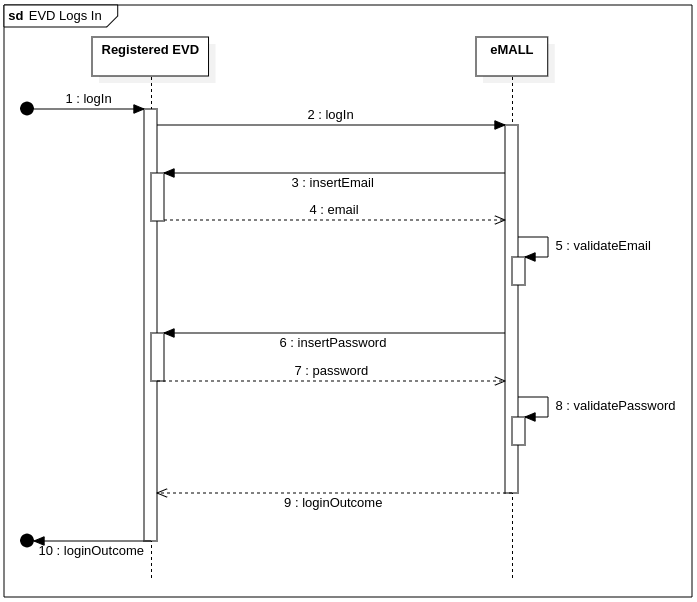
\includegraphics[width=\linewidth]{SequenceDiagrams/evd_logs_in}
        \caption{Registered EVD logs in sequence diagram}
        \label{fig:evd_logs_in}
    \end{center}
\end{figure}

\paragraph{Registered EVD adds an EV}
When the EVD is on his profile page and wants to add a new vehicle to his parking lot, he runs the ``\verb|addVehicle|'' function through the \verb|EVD| \verb|Profile| \verb|Manager| \verb|Service| component.

At first, it asks back to the client to insert the EV information to save in his profile, and then it waits for him.
After the user has sent the information, the component also asks for the nickname to give to the EV\@.
Sending the nickname, the Profile Manager saves the new information by passing them to the \verb|EVDs| \verb|DBMS|\@.
When the DBMS has sent back the ACK message, the \verb|EVD| \verb|Profile| \verb|Manager| \verb|Service| component returns the outcome of the process to the EVD\@.
\begin{figure}[H]
    \begin{center}
        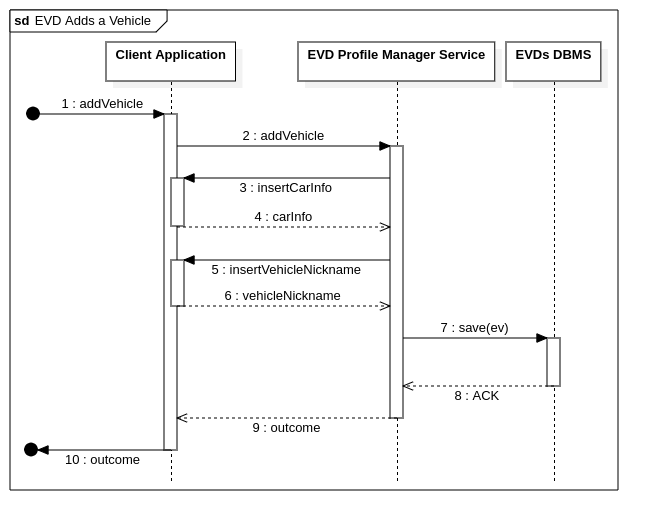
\includegraphics[width=\linewidth]{SequenceDiagrams/evd_adds_a_vehicle}
        \caption{Registered EVD adds an EV sequence diagram}
        \label{fig:evd_adds_vehicle}
    \end{center}
\end{figure}

\paragraph{Registered EVD books a charge}
In eMALL, the EVD can also book a charge in a charging station.
In the sequence diagram, we suppose the \verb|Client| \verb|Application| knows the charging stations he wants to book.
Then, the user calls the ``\verb|bookCharge|'' function of the \verb|Booking| \verb|Service| component, passing the given charging station.

The component needs to know the available timeframes for the charging station, so it waits for the \verb|Sessions| \verb|DBMS| component to process the information.
When it receives the list of timeframes, the \verb|Booking| \verb|Service| asks the user to choose one among them.
Knowing that more than one EVD uses the system, then one timeframe that is at first available might be unavailable when eMALL proceeds with the booking.
To avoid it, the \verb|Booking| \verb|Service| asks for the \verb|Sessions| \verb|DBMS| to check the availability of the chosen timeframe and to lock it if so by calling the ``\verb|isTimeframeAvailable|'' function.

Once the chosen timeframe is locked, the component asks the EVD to confirm the booking - \textit{``}\hyperlink{evdconfirmsbooking}{\textcolor{blue}{\textit{EVD Confirms the Booking}}}\textit{''} sequence diagram.
In the end, the system sends the outcome of the process to the \verb|EVD Client Application|.
\begin{figure}[H]
    \begin{center}
        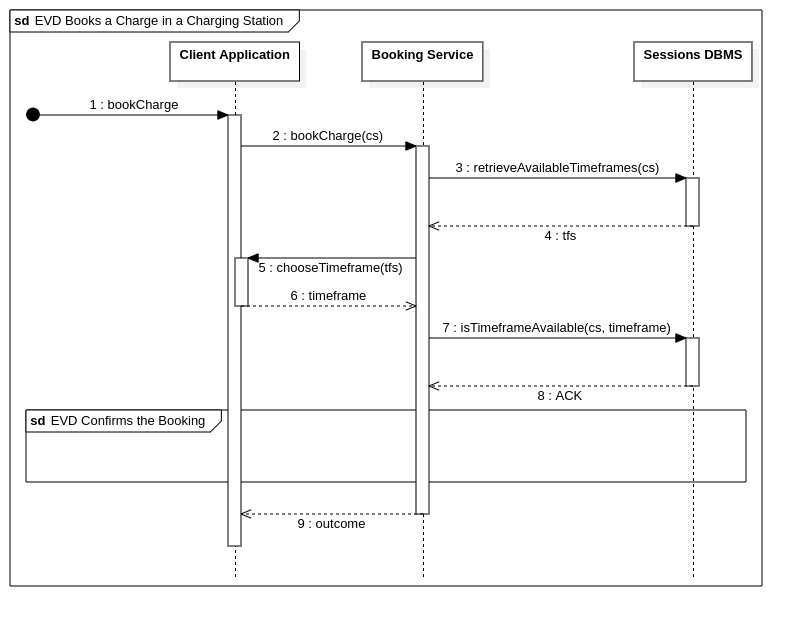
\includegraphics[width=\linewidth]{SequenceDiagrams/edv_books_a_charge_in_a_charging_station}
        \caption{Registered EVD books a charge sequence diagram}
        \label{fig:evd_books_charge_charging_station}
    \end{center}
\end{figure}

\paragraph{\texorpdfstring{\protect\hypertarget{evdconfirmsbooking}{Registered EVD confirms the booking}}{}}
Our system always asks the client to confirm a booking before saving it, so the \verb|Booking| \verb|Service| component receives the client, the charging station where he wants to book, and the timeframe to reserve for the client.
At first, it asks the EVD to confirm the booking and waits for his reply.
Given the confirmation, the \verb|Booking| \verb|Service| runs the ``\verb|addSession|'' function of \verb|Sessions| \verb|DBMS| to add the new booking to the database and orders to the \verb|Calendar| \verb|Service| to add it to the calendar.
After the \verb|Calendar| \verb|Service| has run the ``\verb|saveActivity|'' function of \verb|Calendars| \verb|DBMS|, \verb|Booking| \verb|Service| returns the outcome to the caller.
\begin{figure}[H]
    \begin{center}
        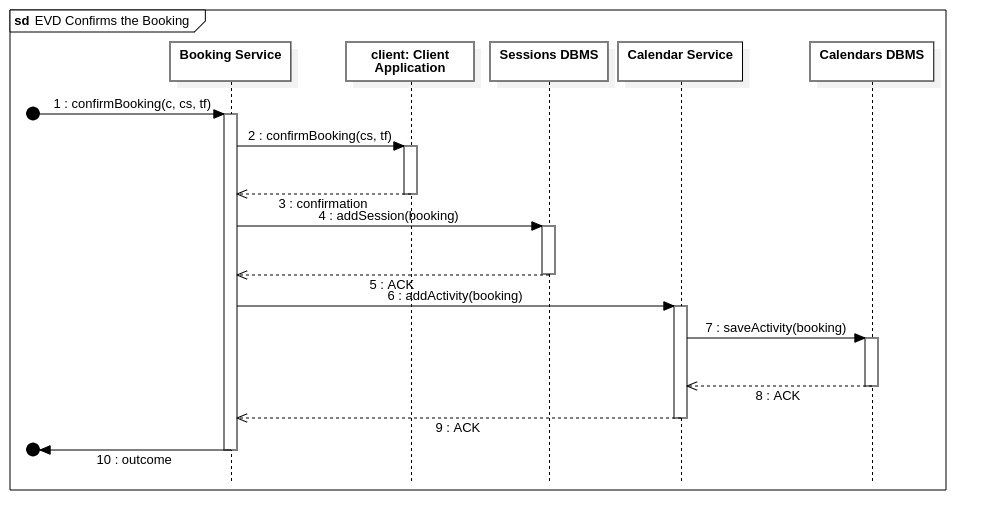
\includegraphics[width=\linewidth]{SequenceDiagrams/evd_confirms_the_booking}
        \caption{Registered EVD confirms the booking sequence diagram}
        \label{fig:evd_confirms_booking}
    \end{center}
\end{figure}

\paragraph{Registered EVD consults a specific promotion that can be redeemed}
An EVD might want to redeem an available promotion in eMALL through his page.
He has to call the ``\verb|redeemPromotion|'' function from the \verb|Promotion| \verb|Service| component, which retrieves all the promotions by running the get function of the list of promotions from the \verb|Promotions| \verb|DBMS|\@.
When the \verb|Promotion| \verb|Service| has received the list, it asks the user to select which promotion he wants to redeem and then asks for a confirmation for its activation.

If the user has decided to proceed with the activation, \verb|Promotion| \verb|Service| initializes the payment by calling the ``\verb|pay|'' function from the \verb|Payment| \verb|Service| component - \textit{``}\hyperlink{evdmakespayment}{\textcolor{blue}{\textit{EVD Makes a Payment}}}\textit{''} sequence diagram.
When the payment successfully ends, the activation process runs through the \verb|EVD| \verb|Profile| \verb|Manager| \verb|Service| component by calling the ``\verb|activate|'' function that receives the paid promotion and the client in input.
The Profile Manager calls the counterpart ``\verb|activate|'' function from the \verb|EVDs| \verb|DBMS|\@.
\begin{figure}[H]
    \begin{center}
        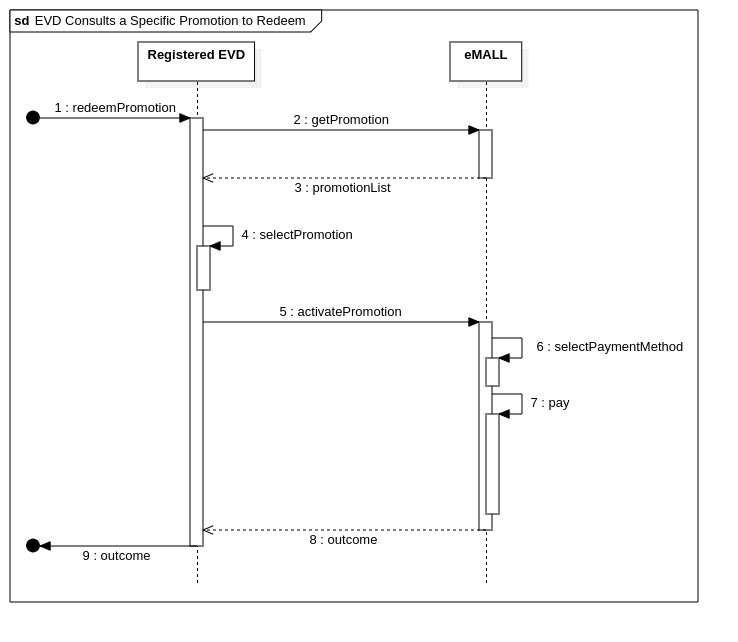
\includegraphics[width=\linewidth]{SequenceDiagrams/evd_consults_a_specific_promotion_to_redeem}
        \caption{Registered EVD consults a specific promotion that can be redeemed sequence diagram}
        \label{fig:evd_consults_specific_promotion_to_redeem}
    \end{center}
\end{figure}

\paragraph{Registered EVD charges his EV}
Now we explain how a charging process evolves in eMALL\@.
At first, we need the EVD to call the function ``\verb|startChargeEV|'' from the \verb|Manage| \verb|Charging| \verb|Session| \verb|Service| component to verify that the current user has booked a charging session.
The service calls so the ``\verb|validateClient|'' from the \verb|Sessions| \verb|DBMS| because it is the only one that can retrieve this information.

The timeframe is not necessary because the system checks at the current time.
If the EVD has booked, the service requests to unlock the charging point to the \verb|Charging| \verb|Station| \verb|Communication| \verb|Service|, which delegates the process to the \verb|Charging| \verb|Point| \verb|System|.
Once the charging point is unlocked, the \verb|Manage| \verb|Charging| \verb|Session| \verb|Service| asks the user to connect his EV and confirm the start of the charging process.

When the EVD confirms, the service asks the \verb|Charging| \verb|Session| \verb|Communication| \verb|Service| to start charging, which delegates to the \verb|Charging| \verb|Point| \verb|System|.
Then, we have a loop sequence where the user asks indirectly for information from the \verb|Charging| \verb|Point| \verb|System| to see the status of his EV's battery.
When the EVD decides to stop the charging process, he communicates it to the \verb|Manage| \verb|Charging| \verb|Session| \verb|Service|, which delegates the decision to the \verb|Charging| \verb|Session| \verb|Communication| \verb|Service|, which orders to stop charging to the \verb|Charging| \verb|Point| \verb|System|.
Finally, the \verb|Manage| \verb|Charging| \verb|Session| \verb|Service| initializes the payment - \textit{``}\hyperlink{evdmakespayment}{\textcolor{blue}{\textit{EVD Makes a Payment}}}\textit{''} sequence diagram - and calls the ``\verb|save|'' function from the \verb|Sessions| \verb|DBMS| to save the EVD session.
\begin{figure}[H]
    \begin{center}
        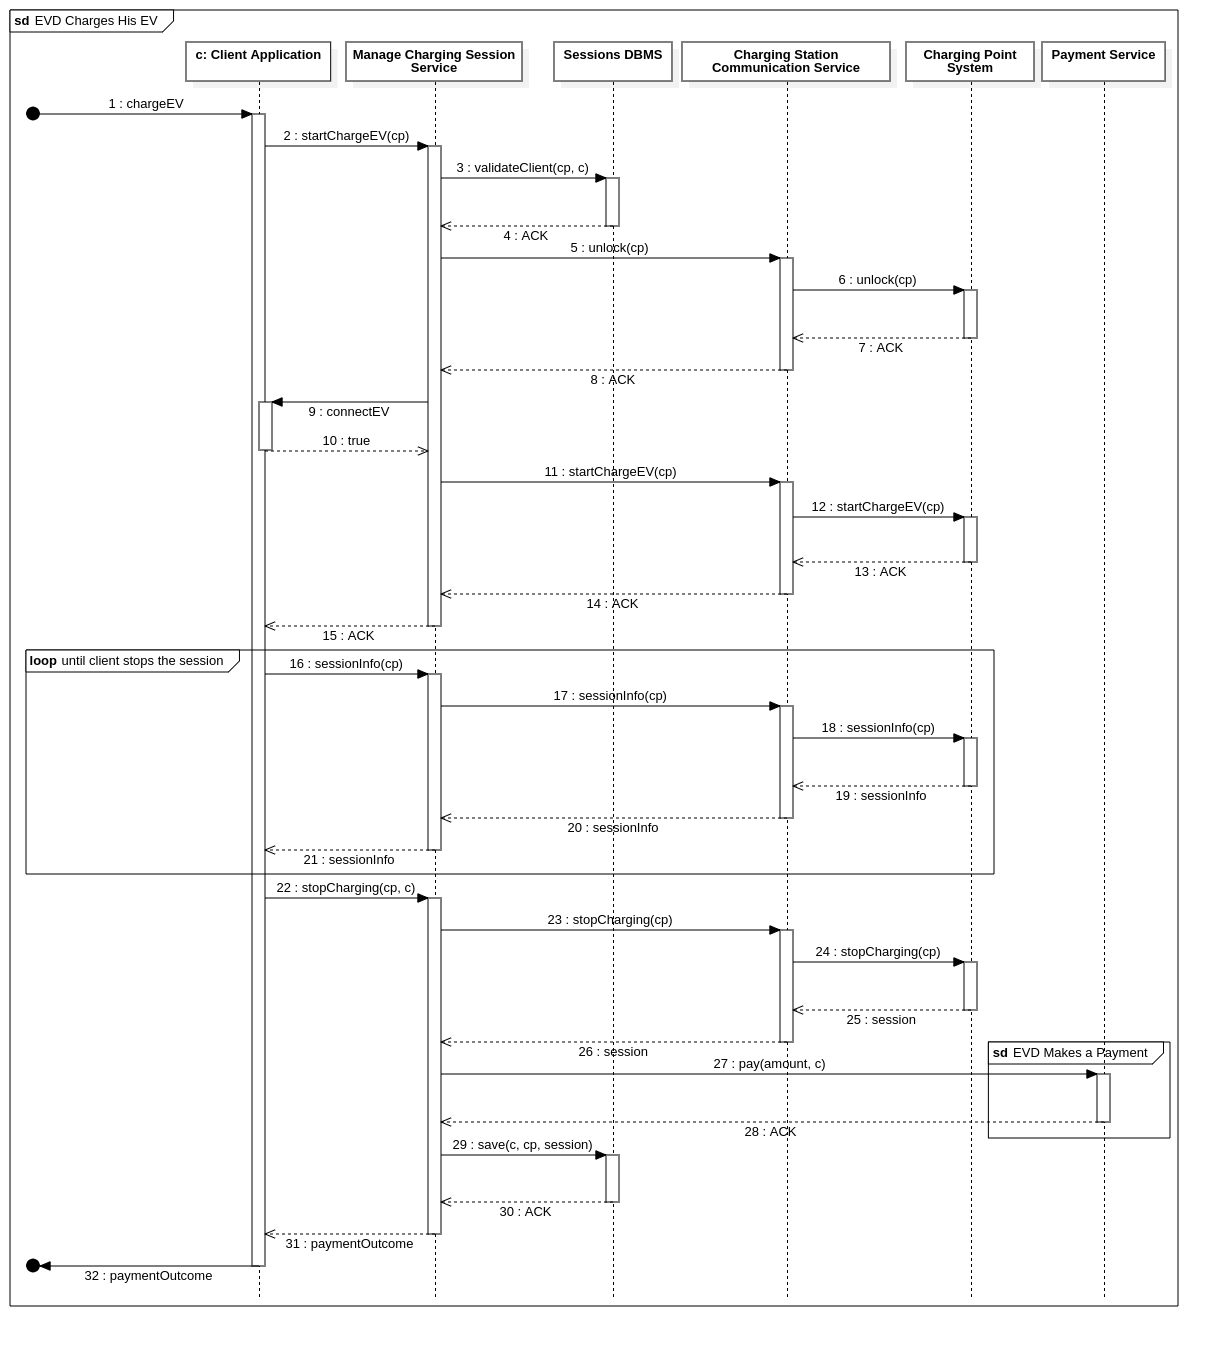
\includegraphics[width=\linewidth]{SequenceDiagrams/edv_charges_his_ev}
        \caption{Registered EVD charges his EV sequence diagram}
        \label{fig:evd_charges_his_ev}
    \end{center}
\end{figure}

\paragraph{\texorpdfstring{\protect\hypertarget{evdmakespayment}{Registered EVD makes a payment}}{}}
When an EVD has to pay, the \verb|Payment| \verb|Service| receives a call with the amount to pay from a client and the client himself in input.
The service asks the \verb|EVD| \verb|Profile| \verb|Manager| \verb|Service| to select a payment method for the given EVD\@.
The Profile Manager asks the \verb|EVDs| \verb|DBMS| for the user's payment methods by calling the ``\verb|getPaymentMethods|'' function and returns the obtained list to the caller.
Finally, the \verb|Payment| \verb|Service| runs the ``\verb|pay|'' function from the \verb|Third-party| \verb|Payment| \verb|Service| with the amount to pay in input.
\begin{figure}[H]
    \begin{center}
        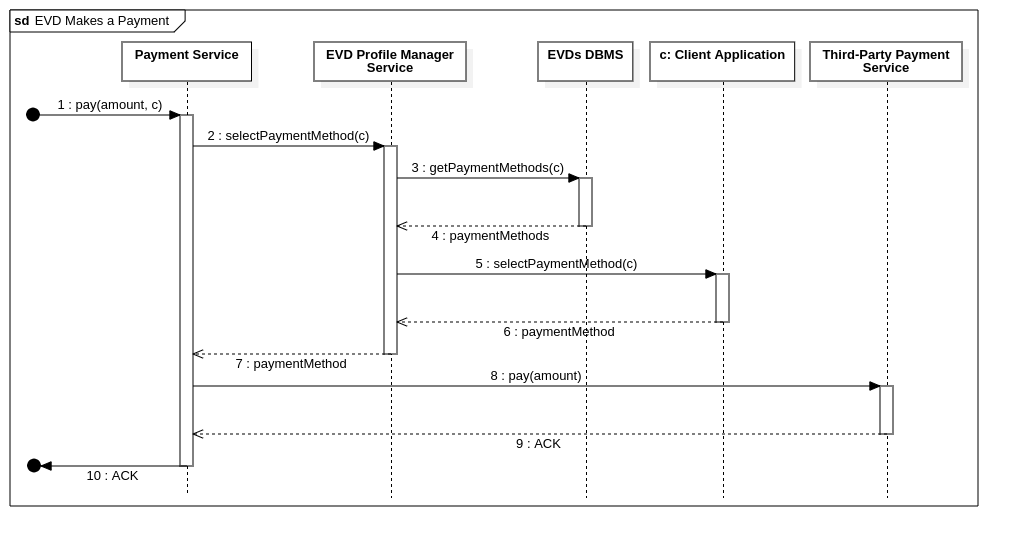
\includegraphics[width=\linewidth]{SequenceDiagrams/evd_makes_a_payment}
        \caption{Registered EVD makes a payment sequence diagram}
        \label{fig:evd_makes_payment}
    \end{center}
\end{figure}

\paragraph{Registered EVD adds a new activity into the calendar and receives suggestions about charging schedule}
When the EVD wants to add a new activity to his calendar, he first opens the calendar section by calling the ``\verb|openCalendar|'' function from the \verb|Calendar| \verb|Service| component, which delegates the call to \verb|Calendars| \verb|DBMS|\@.

Once the user has received the calendar, he can insert the new activity by requesting a form to the \verb|Calendar| \verb|Service| through the ``\verb|insertNewActivity|'' function call.
When the user fills out the form, he sends it to the \verb|Calendar| \verb|Service|, which calls the ``\verb|validateActivity|'' function from the \verb|Calendars| \verb|DBMS| and then the ``\verb|saveActivity|'' function from the same DBMS component.

Finally, the service initializes asynchronously the function ``\verb|findBestSchedule|,'' which computes the best path in reaching the different appointments of the user depending on the battery status of the EV, its capacity, and energy costs - \textit{``}\hyperlink{suggestionfindsschedule}{\textcolor{blue}{\textit{Suggestion Service Finds the Best Schedule}}}\textit{''} sequence diagram.
The call is asynchronous because the service is not essential for the EVD\@.
If the \verb|Suggestion| \verb|Service| component is down, eMALL has to work without it and allow the users to add new activities to their calendars.
\begin{figure}[H]
    \begin{center}
        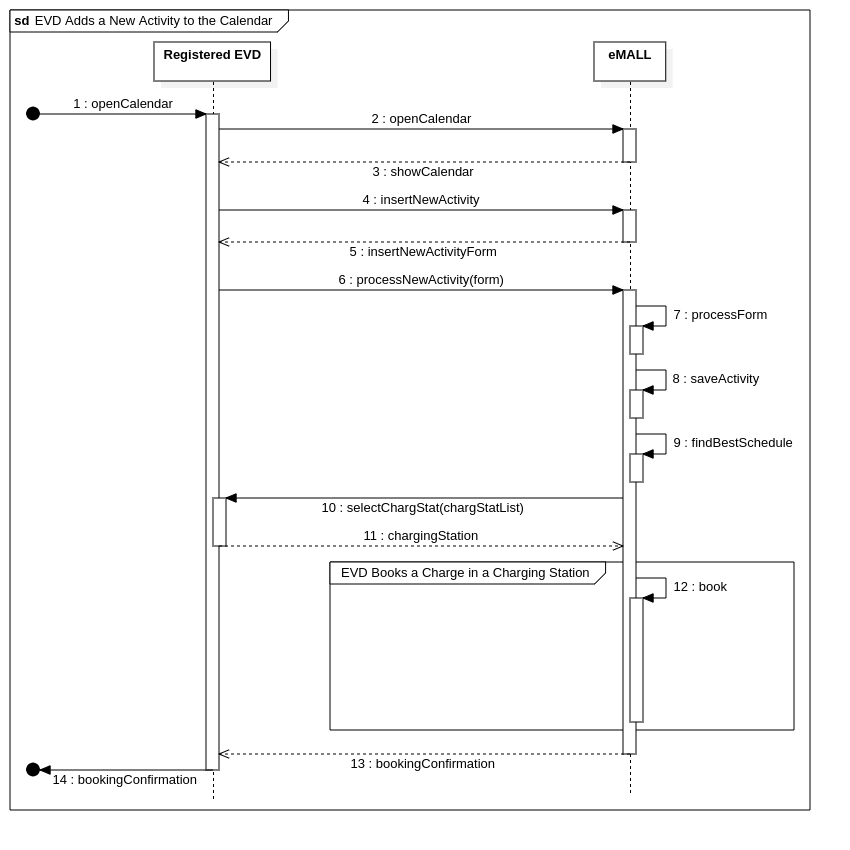
\includegraphics[width=\linewidth]{SequenceDiagrams/evd_adds_a_new_activity_to_the_calendar}
        \caption{Registered EVD adds a new activity into the calendar and receives suggestions about charging schedule sequence diagram}
        \label{fig:evd_adds_new_activity_calendar}
    \end{center}
\end{figure}

\paragraph{\texorpdfstring{\protect\hypertarget{suggestionfindsschedule}{Suggestion service finds the best schedule}}{}}
A feature of eMALL is to provide suggestions in booking charging sessions to allow the EVD to reach the different locations for his activities.
The \verb|Suggestion| \verb|Service| component needs a client id to realize this operation, which is in input to the ``\verb|findBestSchedule|'' function.
The \verb|Suggestion| \verb|Service| is a critical component of eMALL because it communicates with different modules and external APIs.
At first, the ``\verb|findBestSchedule|'' function calls the ``\verb|openCalendar|'' function from the \verb|Calendars| \verb|DBMS| because it needs to know the user activities to compute the optimal suggestion.
When the service gets the calendar, it asks for the client's EV from the \verb|EVDs| \verb|DBMS| and the path the user might follow according to the \verb|Navigator| \verb|System|.
Once the \verb|Suggestion| \verb|Service| has received this information, it runs the ``\verb|optimize|'' function with the EV and the path in input.
The last function orders the \verb|EV| \verb|System| and the \verb|Charging| \verb|Stations| \verb|DBMS| to provide the EV's battery status and the list of charging stations near the given path.
With all the available information, the service asks the \verb|Sessions| \verb|DBMS| which timeframes are available in all the given charging stations.
Finally, the \verb|Suggestion| \verb|Service| component will choose the best timeframe and charging station to book according to the EV information and the activities the EVD will attend.
The process ends by asynchronously calling the ``\verb|confirmBooking|'' function from the \verb|Booking| \verb|Service| component with the client, charging station, and charging point in input - \textit{``}\hyperlink{evdconfirmsbooking}{\textcolor{blue}{\textit{EVD Confirms the Booking}}}\textit{''} sequence diagram.
\begin{figure}[H]
    \begin{center}
        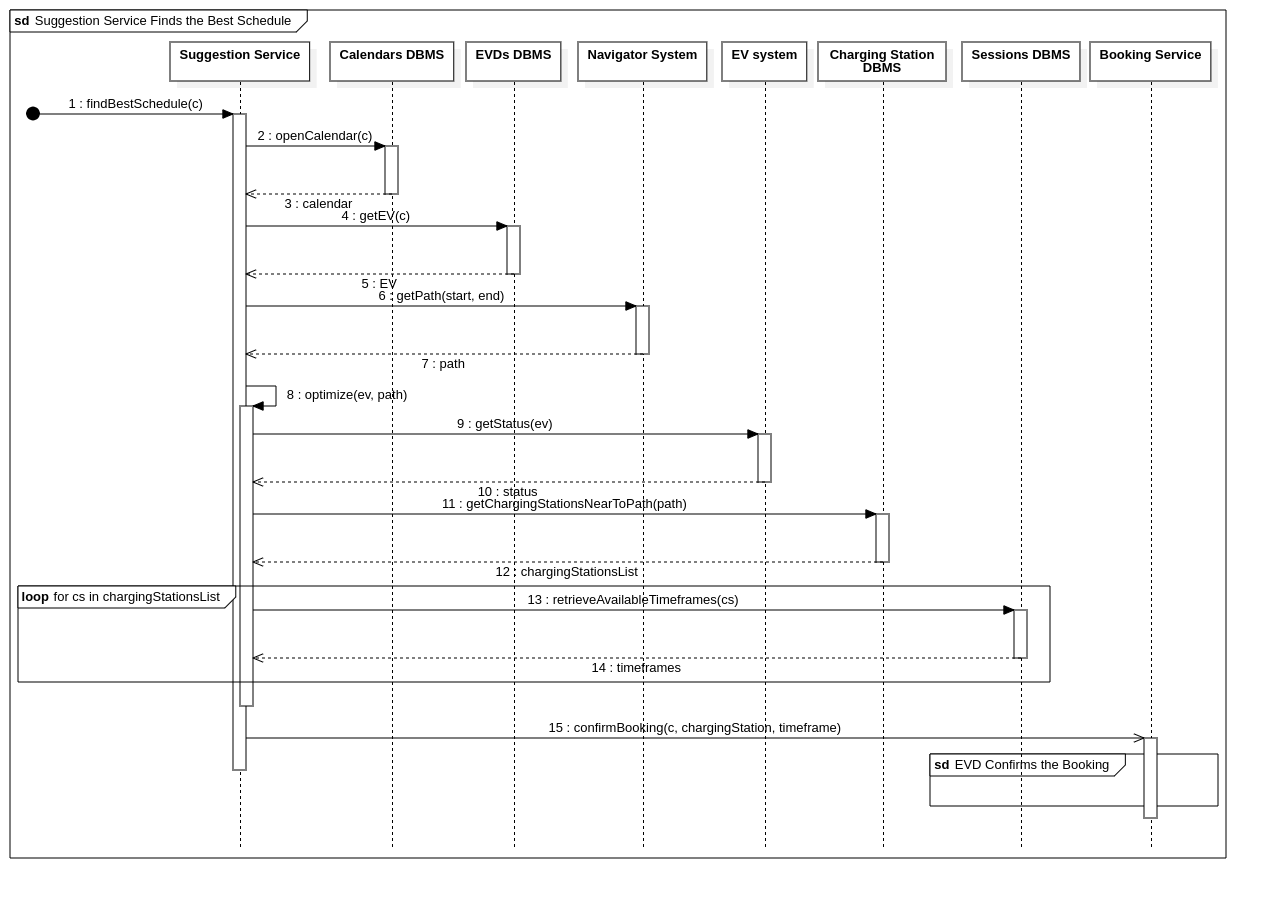
\includegraphics[width=\linewidth]{SequenceDiagrams/suggestion_service_finds_the_best_schedule}
        \caption{Suggestion service finds the best schedule sequence diagram}
        \label{suggestion_service_finds_best_schedule}
    \end{center}
\end{figure}

\paragraph{CPO logs in}
In eMALL, when a CPO wants to log in, he calls the function ``\verb|logInCPO|'' from the \verb|CPO| \verb|Authentication| \verb|Service| component, which calls back the ``\verb|insertInfo|'' function from the \verb|Client| \verb|Application| to retrieve the essential information for the CPO identification, i.e., ID, email, and password.
Once the CPO has sent the information, the Authentication Service runs the ``\verb|validateAccount|'' function from the \verb|CPOs| \verb|DBMS|\@.
If the CPO operator has inserted the correct credentials, he will enter his homepage.
\begin{figure}[H]
    \begin{center}
        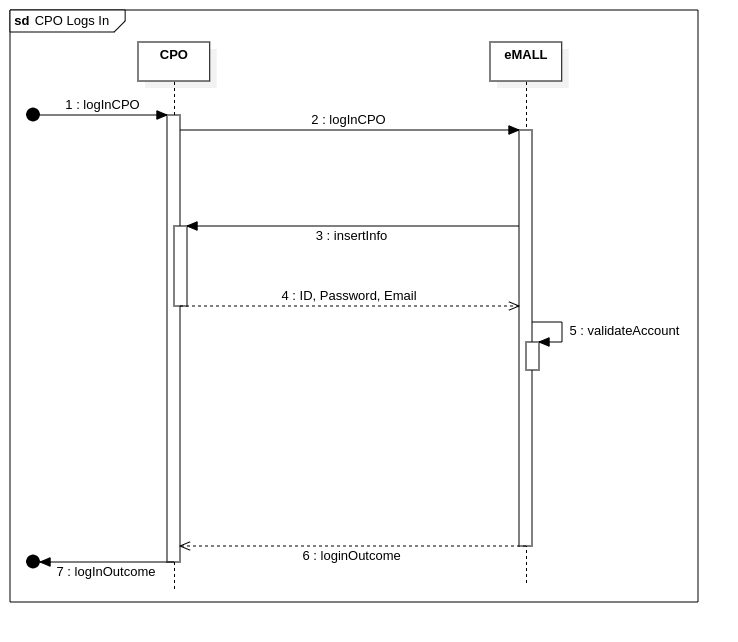
\includegraphics[width=\linewidth]{SequenceDiagrams/cpo_logs_in}
        \caption{CPO logs in sequence diagram}
        \label{cpo_logs_in}
    \end{center}
\end{figure}

\paragraph{CPO sets a fee}
From his homepage, a CPO might want to change the fees of his charging stations.
When he has decided which charging station, he calls the ``\verb|setFee|'' function from the \verb|Charging| \verb|Station| \verb|Manager| \verb|Service| component, which asks the user to insert the new fee to set to the given charging station.
Once the CPO has specified the new fee, the Charging Station Manager runs the ``\verb|updateFee|'' function from the \verb|Charging| \verb|Stations| \verb|DBMS|, which replaces the old fee value with the new one in input.
\begin{figure}[H]
    \begin{center}
        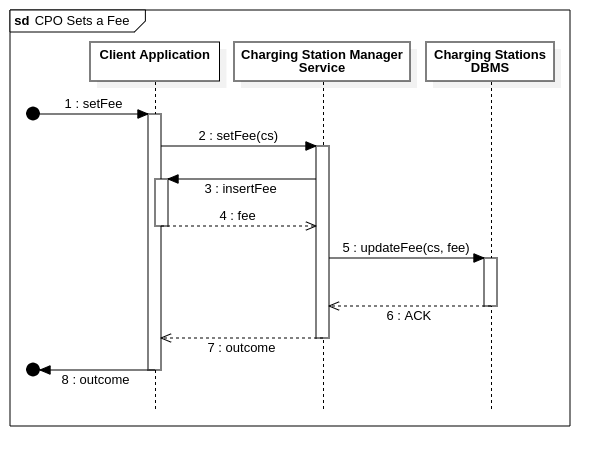
\includegraphics[width=\linewidth]{SequenceDiagrams/cpo_sets_a_fee}
        \caption{CPO sets a fee sequence diagram}
        \label{cpo_sets_fee}
    \end{center}
\end{figure}

\paragraph{CPO adds a charging station}
From his homepage, a CPO can add new charging stations to his profile, so he calls the ``\verb|addChargingStation|'' function from the \verb|Charging| \verb|Station| \verb|Manager| \verb|Service| component.
The service asks the \verb|Client| \verb|Application| to insert the location of the new charging station, its status, the charging costs, and the charging points with their information.
For each piece of information, the service waits for the CPO to reply before proceeding with the new request.
Once the service has received all the information, it passes them to the validate function called from the \verb|Charging| \verb|Stations| \verb|DBMS|\@.
\begin{figure}[H]
    \begin{center}
        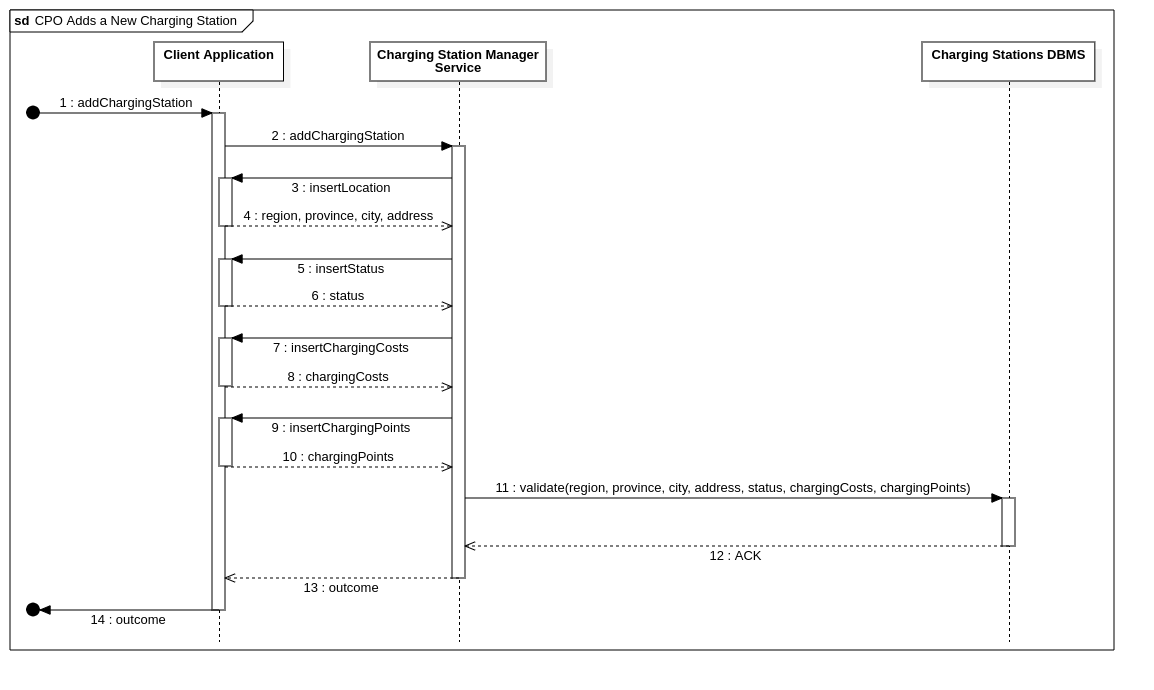
\includegraphics[width=\linewidth]{SequenceDiagrams/cpo_adds_a_new_charging_station}
        \caption{CPO adds a charging station sequence diagram}
        \label{cpo_adds_new_charging_station}
    \end{center}
\end{figure}

\paragraph{CPO adds a charging point}
A CPO can also add new charging points to an existing charging station.
When he chooses this operation, he calls the ``\verb|addChargingPoint|'' function from the \verb|Charging| \verb|Station| \verb|Manager| \verb|Service| component, which asks the \verb|Client| \verb|Application| to enter the charging station where the new charging point has to be added and then the information of the charging point itself.
Once the service has received all the information, it passes them to the validate function called from the \verb|Charging| \verb|Stations| \verb|DBMS|\@.
\begin{figure}[H]
    \begin{center}
        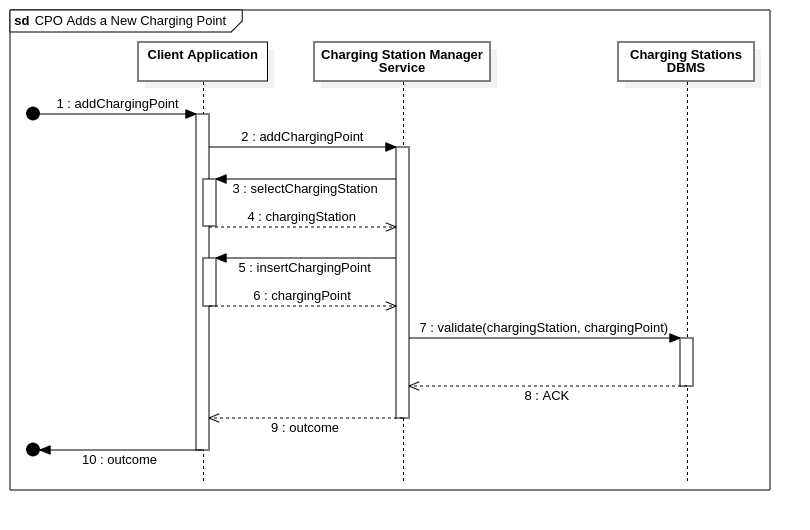
\includegraphics[width=\linewidth]{SequenceDiagrams/cpo_adds_a_new_charging_point}
        \caption{CPO adds a charging point sequence diagram}
        \label{cpo_adds_new_charging_point}
    \end{center}
\end{figure}

\paragraph{CPO changes the metadata of a charging point}
When a CPO wants to edit the metadata of charging points, he calls the ``\verb|updateMetadataChargingPoint|'' from the \verb|Charging| \verb|Station| \verb|Manager| \verb|Service| component with the given charging station in input.
At first, the service asks the \verb|Client| \verb|Application| to select the charging point to edit, so it calls the ``\verb|editMetadataChargingPoint|'' function from the \verb|Client| \verb|Application| that allows the CPO to edit the charging point information.
Once the user has filled out the form, the function returns the new charging point to the Charging Station Manager, which calls the update function with the charging station, the old charging point, and the up-to-date charging point from the \verb|Charging| \verb|Stations| \verb|DBMS|\@.
\begin{figure}[H]
    \begin{center}
        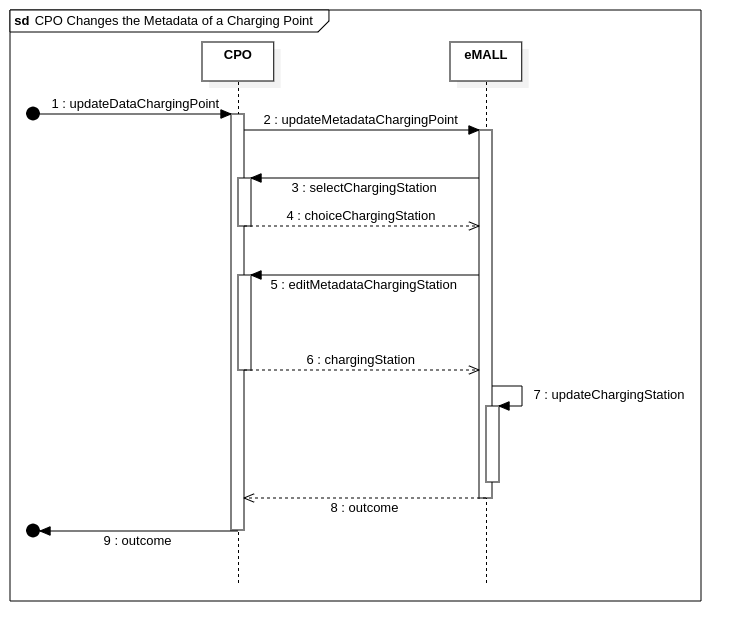
\includegraphics[width=\linewidth]{SequenceDiagrams/cpo_changes_the_metadata_of_a_charging_point}
        \caption{CPO changes the metadata of a charging point sequence diagram}
        \label{cpo_changes_metadata_of_charging_point}
    \end{center}
\end{figure}

\paragraph{CPO activates a promotion}
The CPO can define promotions for the EVD\@.
At first, the CPO calls the ``\verb|activatePromotion|'' function from the \verb|Promotion| \verb|Manager| \verb|Service| component, which calls back the ``\verb|definePromotionFeatures|'' from the \verb|Client| \verb|Application|.
The function, as the name suggests, allows the CPO to define the features of the new promotion.
The form is sent to the caller when filled out.
The Promotion Manager processes the result and, if it's correct, calls the function ``\verb|save|'' with the promotion in input from the \verb|Promotions| \verb|DBMS|\@.
If the store is successful, the service calls the ``\verb|initialize|'' function to make the promotion available to EVDs\@.
\begin{figure}[H]
    \begin{center}
        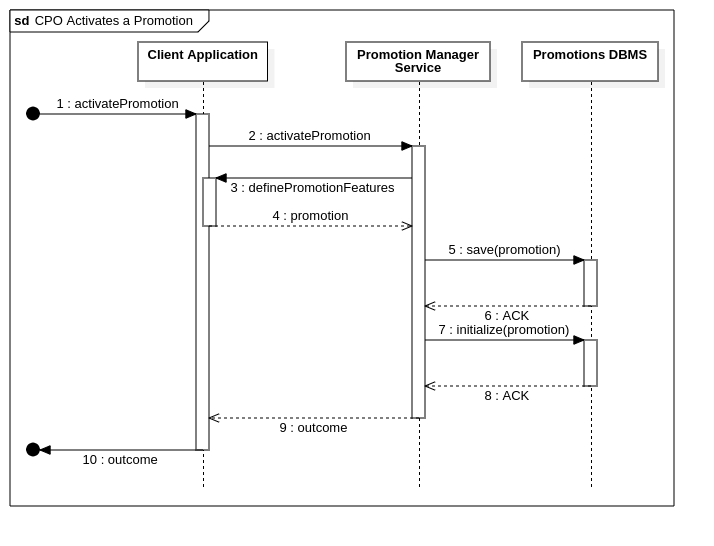
\includegraphics[width=\linewidth]{SequenceDiagrams/cpo_activates_a_promotion}
        \caption{CPO activates a promotion sequence diagram}
        \label{cpo_activates_promotion}
    \end{center}
\end{figure}

\paragraph{CPO plans a maintenance session for a charging station}
A CPO can plan maintenance sessions for his charging station, so here we describe the sequence diagram of the planning process.
At first, the CPO calls the ``\verb|planMaintenanceSession|'' function from the \verb|Charging| \verb|Station| \verb|Manager| \verb|Service| component with the charging station in input.
The service asks the user to fill out the form for the date and hour of the planned maintenance.
Once the CPO returns the form, the Charging Station Manager calls the ``\verb|planMaintenance|'' function from the \verb|Charging| \verb|Station| \verb|Communication| \verb|Service|, which delegates the job to the \verb|Charging| \verb|Point| \verb|System|.
The function notifies the \verb|Charging| \verb|Point| \verb|System| that the charging points of a given charging station will be unavailable on a particular date.
When the Charging Station Manager receives the success notification of the alert, it saves the information into the \verb|Charging| \verb|Stations| \verb|DBMS| by calling the ``\verb|savePlannedMaintenance|'' function with the charging station, date, and hour in input.
\begin{figure}[H]
    \begin{center}
        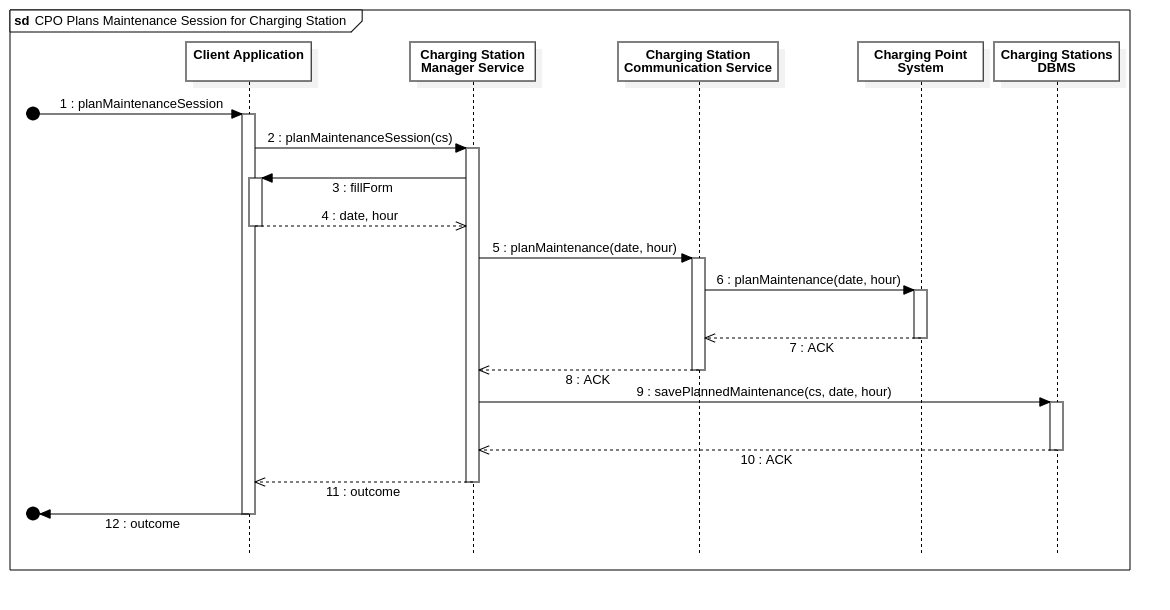
\includegraphics[width=\linewidth]{SequenceDiagrams/cpo_plans_maintenance_session_for_chaging_station}
        \caption{CPO plans a maintenance session for a charging station sequence diagram}
        \label{cpo_plans_maintenance_session_for_charging_station}
    \end{center}
\end{figure}

\paragraph{CPO decides the DSO from which acquire energy}
A CPO can edit his energy provider - DSO - from his homepage.
At first, he calls the ``\verb|setDSOAcquireEnergy|'' function from the \verb|DSO| \verb|Manager| \verb|Service| with the CPO's identifier in input.
The DSO Manager orders the \verb|DSO| \verb|Communication| \verb|Module| to return the list of all the DSOs available in eMALL\@.
When the list is ready, the DSO Manager asks the client to select the DSO from the list, and then it runs the ``\verb|activateDSO|'' function of the \verb|DSO| \verb|Communication| \verb|Module|, which alerts the DSO that a new CPO will acquire energy from it.
After the alert, the service calls the ``\verb|update|'' function from the \verb|CPO| \verb|Profile| \verb|Manager| \verb|Service|, which delegates to the counterpart ``\verb|update|'' function of the \verb|CPOs| \verb|DBMS| to store the new relationship.
The process ends by notifying the \verb|Client| \verb|Application| about the successful ending of the operation.
\begin{figure}[H]
    \begin{center}
        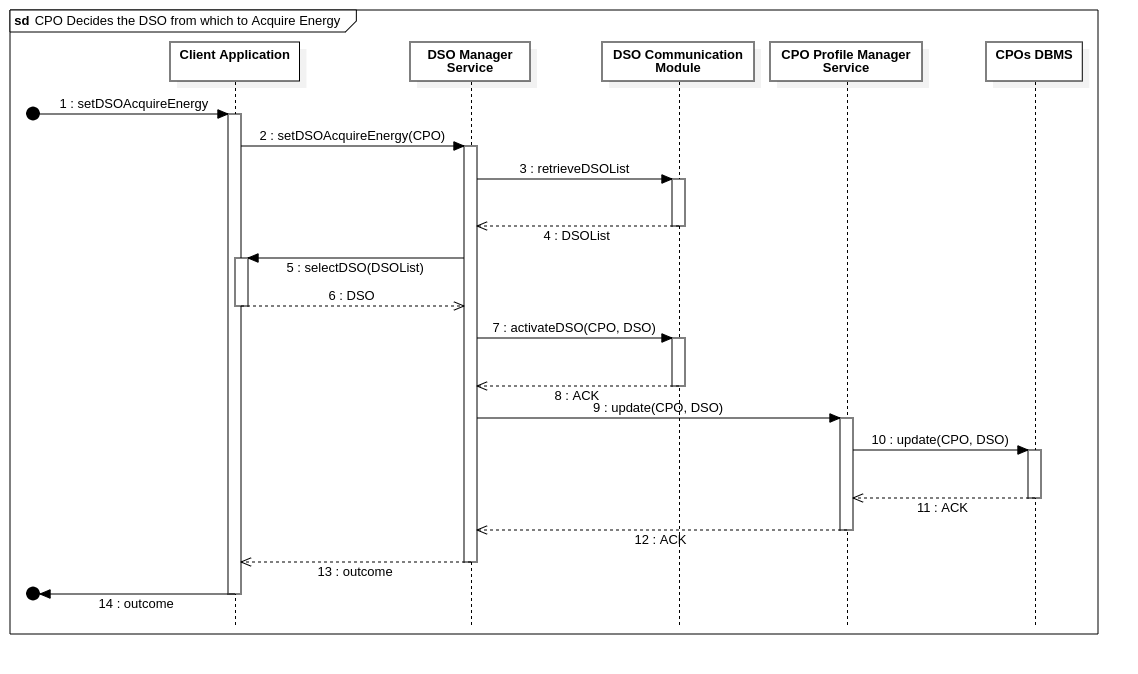
\includegraphics[width=\linewidth]{SequenceDiagrams/cpo_decides_the_dso_from_which_to_acquire_energy}
        \caption{CPO decides the DSO from which acquire energy sequence diagram}
        \label{cpo_decides_dso_from_which_acquire_energy}
    \end{center}
\end{figure}

\newpage


\section{Component Interfaces}
\label{sec: component_interfaces}%
Component interfaces are described as follows.

\paragraph{Booking Service.}
\begin{itemize}
    \item \verb|bookCharge(cs:ChargingStation):boolean|
    \item \verb|confirmBooking(c:Client, cs:ChargingStation, t:Timeframe):boolean|
\end{itemize}

\paragraph{Calendar Service.}
\begin{itemize}
    \item \verb|addActivity(b:Booking):boolean|
    \item \verb|openCalendar(c:Client):Calendar|
    \item \verb|insertNewActivity():Form|
    \item \verb|processForm(f:Form):boolean|
\end{itemize}

\paragraph{Charging Station Communication Service.}
\begin{itemize}
    \item \verb|unlock(cp:ChargingPoint):boolean|
    \item \verb|startChargeEV(cp:ChargingPoint):boolean|
    \item \verb|sessionInfo(cp:ChargingPoint):Session|
    \item \verb|stopCharging(cp:ChargingPoint):Session|
    \item \verb|planMaintenance(d:DateTime)|
\end{itemize}

\paragraph{Charging Station Manager Service.}
\begin{itemize}
    \item \verb|setFee(cs:ChargingStation):boolean|
    \item \verb|addChargingStation(c:Client):boolean|
    \item \verb|addChargingPoint(c:Client):boolean|
    \item \verb|updateMetadataChargingPoint(cs:ChargingStation):boolean|
    \item \verb|activatePromotion(c:Client):boolean|
    \item \verb|planMaintenanceSession(cs:ChargingStation):boolean|
\end{itemize}

\paragraph{CPO Authentication Service.}
\begin{itemize}
    \item \verb|logInCPO():boolean|
\end{itemize}

\paragraph{CPO Profile Manager Service.}
\begin{itemize}
    \item \verb|update(c:Client, dso:DSO):boolean|
\end{itemize}

\paragraph{DSO Manager Service.}
\begin{itemize}
    \item \verb|setDSOAcquireEnergy(c:Client):boolean|
\end{itemize}

\paragraph{EVD Authentication Service.}
\begin{itemize}
    \item \verb|logIn():boolean|
\end{itemize}

\paragraph{EVD Profile Manager Service.}
\begin{itemize}
    \item \verb|addVehicle(c:Client):boolean|
    \item \verb|activate(c:Client, p:Promotion):boolean|
    \item \verb|selectPaymentMethod(c:Client):PaymentMethod|
\end{itemize}

\paragraph{Explore Stations Service.}
\begin{itemize}
    \item \verb|showMap(p:Position):WorldMap|
    \item \verb|showChargingStation(csId:String):ChargingStation|
\end{itemize}

\paragraph{Manage Charging Session Service.}
\begin{itemize}
    \item \verb|startChargeEV(cp:ChargingPoint, c:Client):boolean|
    \item \verb|sessionInfo(cp:ChargingPoint):Session|
    \item \verb|stopCharging(cp:ChargingPoint, c:Client):boolean|
\end{itemize}

\paragraph{Payment Service.}
\begin{itemize}
    \item \verb|pay(a:float, c:Client):boolean|
\end{itemize}

\paragraph{Promotion Manager Service.}
\begin{itemize}
    \item \verb|activatePromotion(c:Client):boolean|
\end{itemize}

\paragraph{Promotion Service.}
\begin{itemize}
    \item \verb|redeemPromotion(c:Client):boolean|
    \item \verb|activate(c:Client, p:Promotion):boolean|
\end{itemize}

\paragraph{Registration Service.}
\begin{itemize}
    \item \verb|register():boolean|
\end{itemize}

\paragraph{Suggestion Service.}
\begin{itemize}
    \item \verb|findBestSchedule(c:Client)|
    \item \verb|optimize(ev:EV, path:Path):(ChargingStation, Timeframe)|
\end{itemize}


\section{Selected Architectural Styles and Patterns}
\label{sec: patterns}%
The \verb|eMALL| system offers functionalities to both EVDs and CPOs.
The second ones represent companies that use the system to manage their business goals.
For this reason, we choose to adopt a microservices architecture. \\
The following list describes the key benefits of the choice:
\begin{itemize}
    \item \textbf{Technology heterogeneity.} With a system composed of multiple, collaborating services, we can decide to use different
    technologies inside each one.
    This allows to pick the right tool for each job.
    As shown in the previous sections, it is shown a wide variety of functionalities.
    So, it is good for the system to use different programming languages and tools depending on the characteristics of
    the module in question.
    \item \textbf{Scalability.} Microservices are designed to be independently deployable and scalable.
    \item \textbf{Availability.} If a service fails, the rest of system keeps running.
    For this reason, is easier to maintain modules that present problems still guaranteeing all the other functionalities
    of the system.
    \item \textbf{Ease of deployment.} With microservices, it is possible to make a change to a single service and deploy
    it independently of the rest of the system.
    If problems occur, they can be identified, isolated, and corrected quicker, without the need of halting the whole system.
\end{itemize}


\section{Other Design Decisions}
\label{sec: other_design_decisions}%

\subsection{Client-Server architecture}
\label{subsec:client_server_architecture}%
The \verb|eMALL| system adopts a 3-tier client-server architecture.
So, the system is divided into three main components: the client, the server, and the databases.
The client represents the front-end user interface, and it is the tool used by users to communicate with the system.
The server is the back-end platform, which receives users' requests, elaborates answers, and stores data.
This design decision has different key benefits: the server can handle several requests simultaneously.
Additionally, it is easier to guarantee the security and integrity of the stored data,
given that the databases are separated from the business logic and users.
Finally, it facilitates maintenance and updates of the parts of the system, given that client and server can be handled independently.

\subsection{Thin client}
\label{subsec:thin_client}%
The mobile app and the web page that will be used by users act as a client, sending requests to the server and receiving responses,
while the server handles the heavy lifting of processing and storing data.
Given the microservices architecture we adopted, the client will communicate to defined offered services according to its needs.
So, the client will be lightweight and easy to use since it doesn't need to store and process large amounts of data.
Another benefit the system enjoys from the thin client design decision is an increase in the system's security
since all the information is processed and stored on the server rather than on the client device.

\subsection{Shared databases}
\label{subsec:shared_databases}%
We decided to introduce databases that will be shared by several services, as already shown in the deployment view section.
The choice relies on several services working on the same kind of data.
The possibility of having only one database shared entirely by services could have introduced strong dependencies between modules.
In the same way, introducing one database for each service and replicating information where needed would have been more expensive.
Considering the system's requirements, sharing databases between modules is, instead, a good point of balance.